%6_fibonacci.tex
%notes for the course PandA2 COMS10001 taught at the University of Bristol
%2015 Conor Houghton conor.houghton@bristol.ac.uk

%To the extent possible under law, the author has dedicated all copyright 
%and related and neighboring rights to these notes to the public domain 
%worldwide. These notes are distributed without any warranty. 


\documentclass[11pt,a4paper]{scrartcl}
\typearea{12}
\usepackage{graphicx}
\usepackage{listings}
\lstset{language=C}
\pagestyle{headings}
\markright{COMS10001 - PandA2 5\_fibonacci - Conor}
\begin{document}

\subsection*{5 The interesting case of the Fibonacci sequence}

Although it is now associated with Leonardo Fibonacci, who wrote about
it in the thirteenth century, the Fibonacci sequence was described in
Indian poetry books from the earliest times. It remains interesting
for number theoretic reasons, for example, it is related to the so
called Golden Mean. One of Alan Turing's interests at the end of his
life was in Fibonacci Phyllotaxis.

The Fibonacci sequence is defined recursively. Using a notation where
the $n$th Fibonacci number is $F(n)$ then the sequence is defined as
having $F(0)=0$, $F(1)=1$ and the $n$th element given by
\begin{equation}
F(n)=F(n-1)+F(n-2)
\end{equation}
This means that if you know all the elements below $F(n)$ you can work
out $F(n)$; since you know $F(0)$ and $F(1)$ you can work out all the
$F(n)$ one by one. This isn't the same as having a direct formula, a
\lq{}closed form\rq{} for $F(n)$ in terms of $n$. If you want
$F(100)$, say, you need to first work out $F(2)$, $F(3)$ and so on all
the way up to $F(98)$ and $F(99)$. In fact, if you try this you'll
find $F(100)$ is very large. The first few terms are
\begin{eqnarray}
F(2)&=&1+0=1\cr
F(3)&=&1+1=2\cr
F(4)&=&2+1=3\cr
F(5)&=&3+2=5\cr
F(6)&=&5+3=8\cr
F(7)&=&8+5=13\cr
F(8)&=&13+8=21\cr
F(9)&=&21+13=34
\end{eqnarray}
and so on. It is in the Encyclopedia of Integer Sequences as {\tt
  http://oeis.org/A000045}. 

The Fibonacci Sequence does have a closed form,
\begin{equation}
F(n)=\frac{\tau^n-(1-\tau)^n}{\sqrt{5}}
\end{equation}
where $\tau=(1+\sqrt{5})/2$. Finding this uses a standard technique in
the study of recursive formula; you substitute $F(n)=r^n$ into the
equation giving
\begin{equation}
r^n=r^{n-1}+r^{n-2}
\end{equation}
Dividing across by $r^{n-2}$ makes this
\begin{equation}
r^2-r-1=0
\end{equation}
and this is solved by
\begin{equation}
r=\frac{1\pm\sqrt{5}}{2}
\end{equation}
or $r=\tau$ and $r=1-\tau$. Since the recursion relation is linear
this means it is solved by
\begin{equation}
F(n)=A \tau^n + B (1-\tau)^n
\end{equation}
for any $A$ and $B$. The values of $A$ and $B$ are fixed by comparing
to the starting values $F(0)=0$ and $F(1)=1$. In fact, because this
involves high powers of irrational numbers, the recursive formula is
more convenient. This is often the case, lots of problems can be more
conveniently expressed in a recursive form. This is particularly true
of problems that are going to be solved on a computer.

An example recursive function for the Fibonacci Sequence is given in
Table~\ref{c_fib_recursion} or in a fancier way in
Table~\ref{c_fib_recursion_fancy}.  As usual with a recursive
function, this function consists of two parts, a base case which
returns fib(n-1)+fib(n-2), and the terminating condition for fib(0)
and fib(1).

\begin{table}
\begin{lstlisting}[numbers=left]
int fib(int n)
{
  if(n==0||n==1){
      return n;
    }

  return fib(n-1)+fib(n-2);

}
\end{lstlisting}
\caption{A recursive function for calculating the Fibonacci
  Sequence. This function can be found included in the program {\tt
    fib\_recursion.c}. If n is 0 or 1 the program returns n, these are
  the stopping conditions, otherwise, the function calls itself with a
  smaller value. The computer will put more and more copies of the
  function on the stack with smaller and smaller values of n until the
  end condition is reached and it passes the values back down to the
  original copy of the function, popping off the stack as it goes,
  until it returns the answer to the main program. This isn't a
  particularly safe implementation, if it is passed a negative integer
  it will never reach a terminating condition and so it will
  eventually overflow the stack and give a segmentation error, this is
  done in {\tt fib\_recursion\_no\-termination.c}; just replacing
  (n==0$\|$n==1) would stop this since then it would always terminate,
  even if the result for $n<0$ is not useful.\label{c_fib_recursion}}
\end{table}


\begin{table}
\begin{lstlisting}[numbers=left]
int fib(int n)
{
  return (n < 2) ? n : fib(n-1) + fib(n-2); 
}
\end{lstlisting}
\caption{A fancier recursive function for calculating the Fibonacci Sequence. This uses the ternary operator. \label{c_fib_recursion_fancy}}
\end{table}

Calculating the run time in the case of Fibonacci is more
difficult. The run time is
\begin{equation}
T(n)=c+T(n-1)+T(n-2)
\end{equation}
so it seems like, apart from a constant, the run time for the
recursive algorithm is itself like a Fibonacci sequence. In fact, it
isn't quite that simple since the Fibonacci sequence has particular
starting values, $F(0)=1$ and $F(1)=1$, but this calculation makes it
clear that the recursive Fibonacci algorithm is $O(\tau^n)$ because
$(1-\tau)^n$ is very small for large $n$. This is terrible. The reason
this algorithm is so poor is that it calculates lots of quantities
lots of times, for example \texttt{fib(n-2)} is calculated when it is
called by \texttt{fib(n)} and when it is called by \texttt{fib(n-1)},
and this extra works gets worse and worse as you go further down.

There are better ways to calculate the Fibonacci sequence!
Table~\ref{c_fib_good_recursion} gives a better algorithm; this
algorithm uses recursion but basically passes along the last two
numbers. It is easy to calculate the running time; on the face of it
\begin{equation}
T(n)=c+T(n-1)
\end{equation}
making this algorithm $O(n)$. Furthermore, this recursion algorithm is
very similar to the more obvious version with a for loop. This isn't
the end of it, there is a $O(\log{n})$ algorithm which won't be
discussed here which rephrases the recursion in terms of matrix
multiplications and uses efficient algorithms to do the matrix
multiplication. 

However, there is another confusing point; Fibonacci numbers get very
large, very quickly. In fact, for large $n$, $F(n)\approx
\tau^n/\sqrt{5}$ so that
\begin{equation}
\log_\tau F(n)\approx n
\end{equation}
or, by the laws of logs
\begin{equation}
\log_{10} F(n) \approx n\log_{10}\tau \approx 0.2090 n
\end{equation}
In other words, since $\lfloor \log_{10} A\rfloor$ gives the number of
digits in $A$, the funny bracket is \lq{}floor\rq{}, the number
rounded down, $F(n)$ has about $n/5$ digits, or put another way, the
number of digits in $F(n)$ is $O(n)$. A graph of the length of $F(n)$
against $n$ is given in Fig.~\ref{fig_fib_length}. All through our
analysis we assume certain operations, including summing numbers, use
a constant amount of time, but here that clearly breaks down, as $n$
gets higher the time spent adding $F(n-1)$ and $F(n-2)$ is going to
get longer, as is the time spend accessing their storage and over
writing the previous values. This case shows just how complicated
calculating run times can be.

\begin{table}
\begin{lstlisting}[numbers=left]
int fib_r(int n, int a, int b)
{
   if(n==0)
     return a;
   if(n==1)
     return b;
   if(n==2)
     return a+b;
     
     return fib_r(n-1,b,a+b);

}

int fib(int n)
{
  return fib_r(n,0,1);
}
\end{lstlisting}
and here is a table for $n=10$, $\$1$, $\$2$ and $\$3$, the three
columns, represent the first, second and third argument of
factorial(int n, int a, int b) when it is called.\\
\begin{tabular}{l|ll}
$\$1$&$\$2$&$\$3$\\
10&0&1\\
9 &1&1\\
8 &1&2\\
7 &2&3\\
6 &3&5\\
5 &5&8\\
4 &8&13\\
3 &13&21\\
2 &21&34\\
\end{tabular}\\
and then it returns $21+34=55$ which is correct.
\caption{A more efficient algorithm for calculating the Fibonacci
  sequence. This algorithm avoids the wasteful extra recursive calls
  that were a feature of the previous Fibonacci function. It does
  lose some of the naturalness though, the recursive structure is
  less obvious and it looks more like an attempt to shoe-horn the
  for-loop form into a recursive function. The for-loop form is given
  in Table~\ref{c_fib_for_loop}. \label{c_fib_good_recursion}}
\end{table}


\begin{table}
\begin{lstlisting}[numbers=left]
int fib(int n)
{
  if(n<2)
     return n;
  
  int last=1, old_last=0;
  int i;

  for(i=2;i<=n;i++){
        int temp=last;
        last=last+old_last;
        old_last=temp;
      }
  return last;
}
\end{lstlisting}

\caption{A simple algorithm for calculating Fibonacci numbers, this is implemented as part of {\tt fib\_loop.c}. \label{c_fib_for_loop}}
\end{table}


\begin{figure}
% GNUPLOT: LaTeX picture with Postscript
\begingroup
  \makeatletter
  \providecommand\color[2][]{%
    \GenericError{(gnuplot) \space\space\space\@spaces}{%
      Package color not loaded in conjunction with
      terminal option `colourtext'%
    }{See the gnuplot documentation for explanation.%
    }{Either use 'blacktext' in gnuplot or load the package
      color.sty in LaTeX.}%
    \renewcommand\color[2][]{}%
  }%
  \providecommand\includegraphics[2][]{%
    \GenericError{(gnuplot) \space\space\space\@spaces}{%
      Package graphicx or graphics not loaded%
    }{See the gnuplot documentation for explanation.%
    }{The gnuplot epslatex terminal needs graphicx.sty or graphics.sty.}%
    \renewcommand\includegraphics[2][]{}%
  }%
  \providecommand\rotatebox[2]{#2}%
  \@ifundefined{ifGPcolor}{%
    \newif\ifGPcolor
    \GPcolorfalse
  }{}%
  \@ifundefined{ifGPblacktext}{%
    \newif\ifGPblacktext
    \GPblacktexttrue
  }{}%
  % define a \g@addto@macro without @ in the name:
  \let\gplgaddtomacro\g@addto@macro
  % define empty templates for all commands taking text:
  \gdef\gplbacktext{}%
  \gdef\gplfronttext{}%
  \makeatother
  \ifGPblacktext
    % no textcolor at all
    \def\colorrgb#1{}%
    \def\colorgray#1{}%
  \else
    % gray or color?
    \ifGPcolor
      \def\colorrgb#1{\color[rgb]{#1}}%
      \def\colorgray#1{\color[gray]{#1}}%
      \expandafter\def\csname LTw\endcsname{\color{white}}%
      \expandafter\def\csname LTb\endcsname{\color{black}}%
      \expandafter\def\csname LTa\endcsname{\color{black}}%
      \expandafter\def\csname LT0\endcsname{\color[rgb]{1,0,0}}%
      \expandafter\def\csname LT1\endcsname{\color[rgb]{0,1,0}}%
      \expandafter\def\csname LT2\endcsname{\color[rgb]{0,0,1}}%
      \expandafter\def\csname LT3\endcsname{\color[rgb]{1,0,1}}%
      \expandafter\def\csname LT4\endcsname{\color[rgb]{0,1,1}}%
      \expandafter\def\csname LT5\endcsname{\color[rgb]{1,1,0}}%
      \expandafter\def\csname LT6\endcsname{\color[rgb]{0,0,0}}%
      \expandafter\def\csname LT7\endcsname{\color[rgb]{1,0.3,0}}%
      \expandafter\def\csname LT8\endcsname{\color[rgb]{0.5,0.5,0.5}}%
    \else
      % gray
      \def\colorrgb#1{\color{black}}%
      \def\colorgray#1{\color[gray]{#1}}%
      \expandafter\def\csname LTw\endcsname{\color{white}}%
      \expandafter\def\csname LTb\endcsname{\color{black}}%
      \expandafter\def\csname LTa\endcsname{\color{black}}%
      \expandafter\def\csname LT0\endcsname{\color{black}}%
      \expandafter\def\csname LT1\endcsname{\color{black}}%
      \expandafter\def\csname LT2\endcsname{\color{black}}%
      \expandafter\def\csname LT3\endcsname{\color{black}}%
      \expandafter\def\csname LT4\endcsname{\color{black}}%
      \expandafter\def\csname LT5\endcsname{\color{black}}%
      \expandafter\def\csname LT6\endcsname{\color{black}}%
      \expandafter\def\csname LT7\endcsname{\color{black}}%
      \expandafter\def\csname LT8\endcsname{\color{black}}%
    \fi
  \fi
  \setlength{\unitlength}{0.0500bp}%
  \begin{picture}(7200.00,5040.00)%
    \gplgaddtomacro\gplbacktext{%
      \csname LTb\endcsname%
      \put(1210,704){\makebox(0,0)[r]{\strut{} 0}}%
      \put(1210,1518){\makebox(0,0)[r]{\strut{} 5000}}%
      \put(1210,2332){\makebox(0,0)[r]{\strut{} 10000}}%
      \put(1210,3147){\makebox(0,0)[r]{\strut{} 15000}}%
      \put(1210,3961){\makebox(0,0)[r]{\strut{} 20000}}%
      \put(1210,4775){\makebox(0,0)[r]{\strut{} 25000}}%
      \put(1342,484){\makebox(0,0){\strut{} 0}}%
      \put(2707,484){\makebox(0,0){\strut{} 25000}}%
      \put(4072,484){\makebox(0,0){\strut{} 50000}}%
      \put(5438,484){\makebox(0,0){\strut{} 75000}}%
      \put(6803,484){\makebox(0,0){\strut{} 100000}}%
      \put(176,2739){\rotatebox{-270}{\makebox(0,0){\strut{}length}}}%
      \put(4072,154){\makebox(0,0){\strut{}iterations}}%
    }%
    \gplgaddtomacro\gplfronttext{%
      \csname LTb\endcsname%
      \put(5816,4602){\makebox(0,0)[r]{\strut{}number length in digits}}%
    }%
    \gplbacktext
    \put(0,0){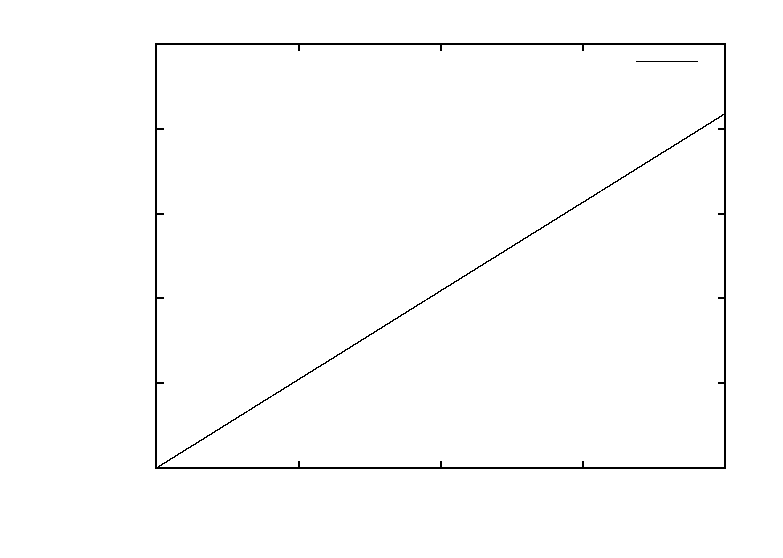
\includegraphics{fib_length.eps}}%
    \gplfronttext
  \end{picture}%
\endgroup

\caption{A plot of the length of $F(n)$ in digits against $n$. \label{fig_fib_length}}
\end{figure}


\end{document}
